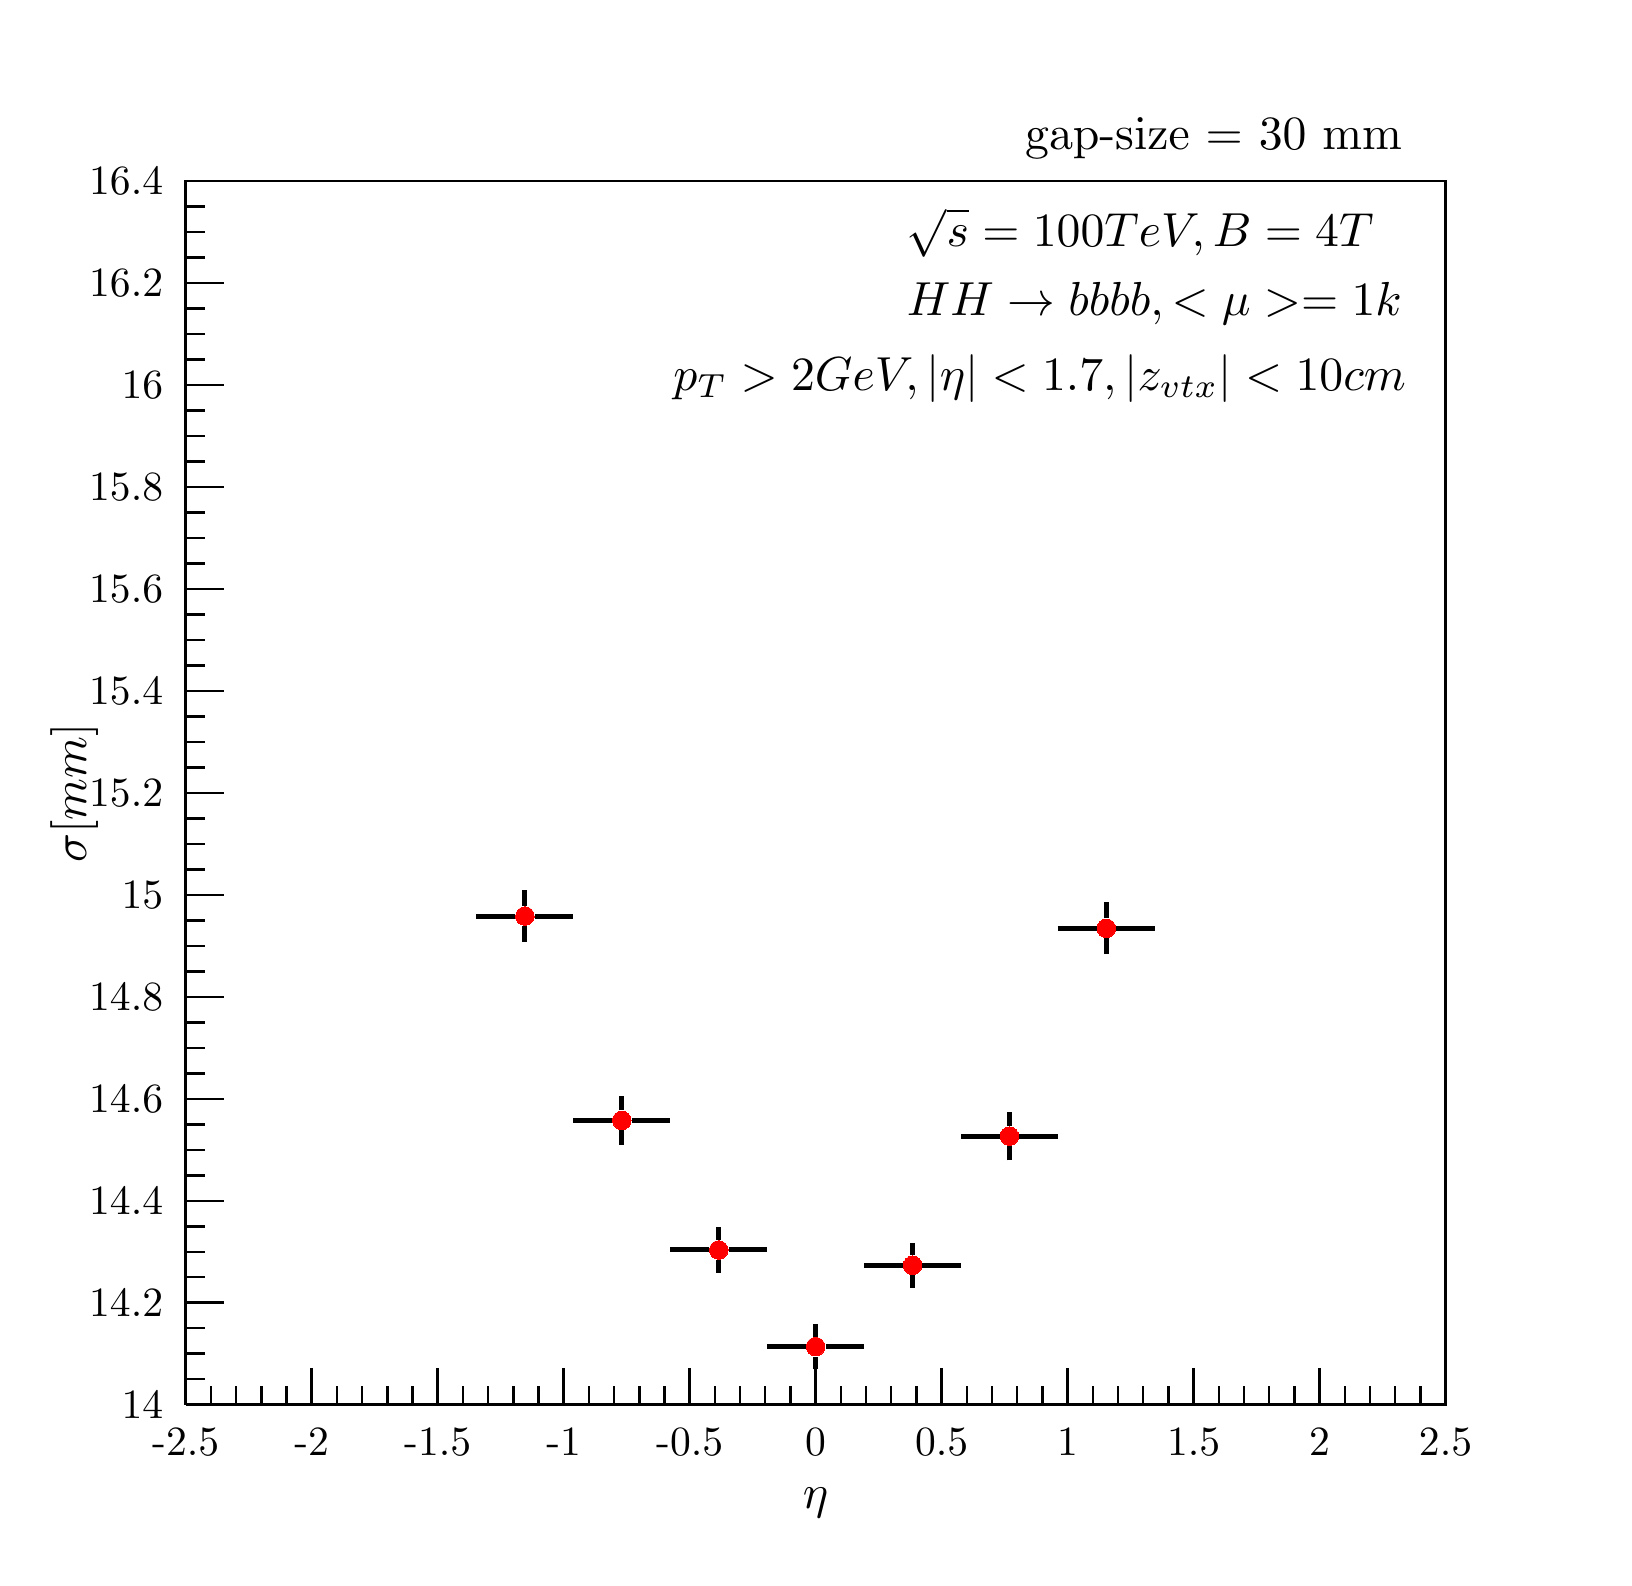
\begin{tikzpicture}
\pgfdeclareplotmark{cross} {
\pgfpathmoveto{\pgfpoint{-0.3\pgfplotmarksize}{\pgfplotmarksize}}
\pgfpathlineto{\pgfpoint{+0.3\pgfplotmarksize}{\pgfplotmarksize}}
\pgfpathlineto{\pgfpoint{+0.3\pgfplotmarksize}{0.3\pgfplotmarksize}}
\pgfpathlineto{\pgfpoint{+1\pgfplotmarksize}{0.3\pgfplotmarksize}}
\pgfpathlineto{\pgfpoint{+1\pgfplotmarksize}{-0.3\pgfplotmarksize}}
\pgfpathlineto{\pgfpoint{+0.3\pgfplotmarksize}{-0.3\pgfplotmarksize}}
\pgfpathlineto{\pgfpoint{+0.3\pgfplotmarksize}{-1.\pgfplotmarksize}}
\pgfpathlineto{\pgfpoint{-0.3\pgfplotmarksize}{-1.\pgfplotmarksize}}
\pgfpathlineto{\pgfpoint{-0.3\pgfplotmarksize}{-0.3\pgfplotmarksize}}
\pgfpathlineto{\pgfpoint{-1.\pgfplotmarksize}{-0.3\pgfplotmarksize}}
\pgfpathlineto{\pgfpoint{-1.\pgfplotmarksize}{0.3\pgfplotmarksize}}
\pgfpathlineto{\pgfpoint{-0.3\pgfplotmarksize}{0.3\pgfplotmarksize}}
\pgfpathclose
\pgfusepathqstroke
}
\pgfdeclareplotmark{cross*} {
\pgfpathmoveto{\pgfpoint{-0.3\pgfplotmarksize}{\pgfplotmarksize}}
\pgfpathlineto{\pgfpoint{+0.3\pgfplotmarksize}{\pgfplotmarksize}}
\pgfpathlineto{\pgfpoint{+0.3\pgfplotmarksize}{0.3\pgfplotmarksize}}
\pgfpathlineto{\pgfpoint{+1\pgfplotmarksize}{0.3\pgfplotmarksize}}
\pgfpathlineto{\pgfpoint{+1\pgfplotmarksize}{-0.3\pgfplotmarksize}}
\pgfpathlineto{\pgfpoint{+0.3\pgfplotmarksize}{-0.3\pgfplotmarksize}}
\pgfpathlineto{\pgfpoint{+0.3\pgfplotmarksize}{-1.\pgfplotmarksize}}
\pgfpathlineto{\pgfpoint{-0.3\pgfplotmarksize}{-1.\pgfplotmarksize}}
\pgfpathlineto{\pgfpoint{-0.3\pgfplotmarksize}{-0.3\pgfplotmarksize}}
\pgfpathlineto{\pgfpoint{-1.\pgfplotmarksize}{-0.3\pgfplotmarksize}}
\pgfpathlineto{\pgfpoint{-1.\pgfplotmarksize}{0.3\pgfplotmarksize}}
\pgfpathlineto{\pgfpoint{-0.3\pgfplotmarksize}{0.3\pgfplotmarksize}}
\pgfpathclose
\pgfusepathqfillstroke
}
\pgfdeclareplotmark{newstar} {
\pgfpathmoveto{\pgfqpoint{0pt}{\pgfplotmarksize}}
\pgfpathlineto{\pgfqpointpolar{44}{0.5\pgfplotmarksize}}
\pgfpathlineto{\pgfqpointpolar{18}{\pgfplotmarksize}}
\pgfpathlineto{\pgfqpointpolar{-20}{0.5\pgfplotmarksize}}
\pgfpathlineto{\pgfqpointpolar{-54}{\pgfplotmarksize}}
\pgfpathlineto{\pgfqpointpolar{-90}{0.5\pgfplotmarksize}}
\pgfpathlineto{\pgfqpointpolar{234}{\pgfplotmarksize}}
\pgfpathlineto{\pgfqpointpolar{198}{0.5\pgfplotmarksize}}
\pgfpathlineto{\pgfqpointpolar{162}{\pgfplotmarksize}}
\pgfpathlineto{\pgfqpointpolar{134}{0.5\pgfplotmarksize}}
\pgfpathclose
\pgfusepathqstroke
}
\pgfdeclareplotmark{newstar*} {
\pgfpathmoveto{\pgfqpoint{0pt}{\pgfplotmarksize}}
\pgfpathlineto{\pgfqpointpolar{44}{0.5\pgfplotmarksize}}
\pgfpathlineto{\pgfqpointpolar{18}{\pgfplotmarksize}}
\pgfpathlineto{\pgfqpointpolar{-20}{0.5\pgfplotmarksize}}
\pgfpathlineto{\pgfqpointpolar{-54}{\pgfplotmarksize}}
\pgfpathlineto{\pgfqpointpolar{-90}{0.5\pgfplotmarksize}}
\pgfpathlineto{\pgfqpointpolar{234}{\pgfplotmarksize}}
\pgfpathlineto{\pgfqpointpolar{198}{0.5\pgfplotmarksize}}
\pgfpathlineto{\pgfqpointpolar{162}{\pgfplotmarksize}}
\pgfpathlineto{\pgfqpointpolar{134}{0.5\pgfplotmarksize}}
\pgfpathclose
\pgfusepathqfillstroke
}
\definecolor{c}{rgb}{1,1,1};
\draw [color=c, fill=c] (0,0) rectangle (20,19.4236);
\draw [color=c, fill=c] (2,1.94236) rectangle (18,17.4812);
\definecolor{c}{rgb}{0,0,0};
\draw [c,line width=0.9] (2,1.94236) -- (2,17.4812) -- (18,17.4812) -- (18,1.94236) -- (2,1.94236);
\draw [c,line width=1.8] (6.30769,7.819) -- (6.30769,8.02272);
\draw [c,line width=1.8] (6.30769,8.27335) -- (6.30769,8.47707);
\draw [c,line width=1.8] (5.69231,8.14803) -- (6.18238,8.14803);
\draw [c,line width=1.8] (6.43301,8.14803) -- (6.92308,8.14803);
\definecolor{c}{rgb}{1,0,0};
\foreach \P in {(6.30769,8.14803)}{\draw[mark options={color=c,fill=c},mark size=3.363363pt, line width=0.000000pt, mark=*] plot coordinates {\P};}
\definecolor{c}{rgb}{0,0,0};
\draw [c,line width=1.8] (7.53846,5.24416) -- (7.53846,5.42806);
\draw [c,line width=1.8] (7.53846,5.67869) -- (7.53846,5.86258);
\draw [c,line width=1.8] (6.92308,5.55337) -- (7.41315,5.55337);
\draw [c,line width=1.8] (7.66377,5.55337) -- (8.15385,5.55337);
\definecolor{c}{rgb}{1,0,0};
\foreach \P in {(7.53846,5.55337)}{\draw[mark options={color=c,fill=c},mark size=3.363363pt, line width=0.000000pt, mark=*] plot coordinates {\P};}
\definecolor{c}{rgb}{0,0,0};
\draw [c,line width=1.8] (8.76923,3.61842) -- (8.76923,3.78202);
\draw [c,line width=1.8] (8.76923,4.03264) -- (8.76923,4.19624);
\draw [c,line width=1.8] (8.15385,3.90733) -- (8.64392,3.90733);
\draw [c,line width=1.8] (8.89454,3.90733) -- (9.38461,3.90733);
\definecolor{c}{rgb}{1,0,0};
\foreach \P in {(8.76923,3.90733)}{\draw[mark options={color=c,fill=c},mark size=3.363363pt, line width=0.000000pt, mark=*] plot coordinates {\P};}
\definecolor{c}{rgb}{0,0,0};
\draw [c,line width=1.8] (10,2.38979) -- (10,2.55443);
\draw [c,line width=1.8] (10,2.80505) -- (10,2.96969);
\draw [c,line width=1.8] (9.38461,2.67974) -- (9.87469,2.67974);
\draw [c,line width=1.8] (10.1253,2.67974) -- (10.6154,2.67974);
\definecolor{c}{rgb}{1,0,0};
\foreach \P in {(10,2.67974)}{\draw[mark options={color=c,fill=c},mark size=3.363363pt, line width=0.000000pt, mark=*] plot coordinates {\P};}
\definecolor{c}{rgb}{0,0,0};
\draw [c,line width=1.8] (11.2308,3.42719) -- (11.2308,3.58755);
\draw [c,line width=1.8] (11.2308,3.83818) -- (11.2308,3.99855);
\draw [c,line width=1.8] (10.6154,3.71287) -- (11.1055,3.71287);
\draw [c,line width=1.8] (11.3561,3.71287) -- (11.8462,3.71287);
\definecolor{c}{rgb}{1,0,0};
\foreach \P in {(11.2308,3.71287)}{\draw[mark options={color=c,fill=c},mark size=3.363363pt, line width=0.000000pt, mark=*] plot coordinates {\P};}
\definecolor{c}{rgb}{0,0,0};
\draw [c,line width=1.8] (12.4615,5.04533) -- (12.4615,5.22733);
\draw [c,line width=1.8] (12.4615,5.47795) -- (12.4615,5.65995);
\draw [c,line width=1.8] (11.8462,5.35264) -- (12.3362,5.35264);
\draw [c,line width=1.8] (12.5869,5.35264) -- (13.0769,5.35264);
\definecolor{c}{rgb}{1,0,0};
\foreach \P in {(12.4615,5.35264)}{\draw[mark options={color=c,fill=c},mark size=3.363363pt, line width=0.000000pt, mark=*] plot coordinates {\P};}
\definecolor{c}{rgb}{0,0,0};
\draw [c,line width=1.8] (13.6923,7.66381) -- (13.6923,7.86675);
\draw [c,line width=1.8] (13.6923,8.11737) -- (13.6923,8.32031);
\draw [c,line width=1.8] (13.0769,7.99206) -- (13.567,7.99206);
\draw [c,line width=1.8] (13.8176,7.99206) -- (14.3077,7.99206);
\definecolor{c}{rgb}{1,0,0};
\foreach \P in {(13.6923,7.99206)}{\draw[mark options={color=c,fill=c},mark size=3.363363pt, line width=0.000000pt, mark=*] plot coordinates {\P};}
\definecolor{c}{rgb}{0,0,0};
\draw [c,line width=0.9] (2,1.94236) -- (18,1.94236);
\draw [c,line width=0.9] (2,2.40852) -- (2,1.94236);
\draw [c,line width=0.9] (2.32,2.17544) -- (2.32,1.94236);
\draw [c,line width=0.9] (2.64,2.17544) -- (2.64,1.94236);
\draw [c,line width=0.9] (2.96,2.17544) -- (2.96,1.94236);
\draw [c,line width=0.9] (3.28,2.17544) -- (3.28,1.94236);
\draw [c,line width=0.9] (3.6,2.40852) -- (3.6,1.94236);
\draw [c,line width=0.9] (3.92,2.17544) -- (3.92,1.94236);
\draw [c,line width=0.9] (4.24,2.17544) -- (4.24,1.94236);
\draw [c,line width=0.9] (4.56,2.17544) -- (4.56,1.94236);
\draw [c,line width=0.9] (4.88,2.17544) -- (4.88,1.94236);
\draw [c,line width=0.9] (5.2,2.40852) -- (5.2,1.94236);
\draw [c,line width=0.9] (5.52,2.17544) -- (5.52,1.94236);
\draw [c,line width=0.9] (5.84,2.17544) -- (5.84,1.94236);
\draw [c,line width=0.9] (6.16,2.17544) -- (6.16,1.94236);
\draw [c,line width=0.9] (6.48,2.17544) -- (6.48,1.94236);
\draw [c,line width=0.9] (6.8,2.40852) -- (6.8,1.94236);
\draw [c,line width=0.9] (7.12,2.17544) -- (7.12,1.94236);
\draw [c,line width=0.9] (7.44,2.17544) -- (7.44,1.94236);
\draw [c,line width=0.9] (7.76,2.17544) -- (7.76,1.94236);
\draw [c,line width=0.9] (8.08,2.17544) -- (8.08,1.94236);
\draw [c,line width=0.9] (8.4,2.40852) -- (8.4,1.94236);
\draw [c,line width=0.9] (8.72,2.17544) -- (8.72,1.94236);
\draw [c,line width=0.9] (9.04,2.17544) -- (9.04,1.94236);
\draw [c,line width=0.9] (9.36,2.17544) -- (9.36,1.94236);
\draw [c,line width=0.9] (9.68,2.17544) -- (9.68,1.94236);
\draw [c,line width=0.9] (10,2.40852) -- (10,1.94236);
\draw [c,line width=0.9] (10.32,2.17544) -- (10.32,1.94236);
\draw [c,line width=0.9] (10.64,2.17544) -- (10.64,1.94236);
\draw [c,line width=0.9] (10.96,2.17544) -- (10.96,1.94236);
\draw [c,line width=0.9] (11.28,2.17544) -- (11.28,1.94236);
\draw [c,line width=0.9] (11.6,2.40852) -- (11.6,1.94236);
\draw [c,line width=0.9] (11.92,2.17544) -- (11.92,1.94236);
\draw [c,line width=0.9] (12.24,2.17544) -- (12.24,1.94236);
\draw [c,line width=0.9] (12.56,2.17544) -- (12.56,1.94236);
\draw [c,line width=0.9] (12.88,2.17544) -- (12.88,1.94236);
\draw [c,line width=0.9] (13.2,2.40852) -- (13.2,1.94236);
\draw [c,line width=0.9] (13.52,2.17544) -- (13.52,1.94236);
\draw [c,line width=0.9] (13.84,2.17544) -- (13.84,1.94236);
\draw [c,line width=0.9] (14.16,2.17544) -- (14.16,1.94236);
\draw [c,line width=0.9] (14.48,2.17544) -- (14.48,1.94236);
\draw [c,line width=0.9] (14.8,2.40852) -- (14.8,1.94236);
\draw [c,line width=0.9] (15.12,2.17544) -- (15.12,1.94236);
\draw [c,line width=0.9] (15.44,2.17544) -- (15.44,1.94236);
\draw [c,line width=0.9] (15.76,2.17544) -- (15.76,1.94236);
\draw [c,line width=0.9] (16.08,2.17544) -- (16.08,1.94236);
\draw [c,line width=0.9] (16.4,2.40852) -- (16.4,1.94236);
\draw [c,line width=0.9] (16.72,2.17544) -- (16.72,1.94236);
\draw [c,line width=0.9] (17.04,2.17544) -- (17.04,1.94236);
\draw [c,line width=0.9] (17.36,2.17544) -- (17.36,1.94236);
\draw [c,line width=0.9] (17.68,2.17544) -- (17.68,1.94236);
\draw [c,line width=0.9] (18,2.40852) -- (18,1.94236);
\draw [c,line width=0.9] (18,2.40852) -- (18,1.94236);
\draw [anchor=base] (2,1.30138) node[scale=1.50291, color=c, rotate=0]{-2.5};
\draw [anchor=base] (3.6,1.30138) node[scale=1.50291, color=c, rotate=0]{-2};
\draw [anchor=base] (5.2,1.30138) node[scale=1.50291, color=c, rotate=0]{-1.5};
\draw [anchor=base] (6.8,1.30138) node[scale=1.50291, color=c, rotate=0]{-1};
\draw [anchor=base] (8.4,1.30138) node[scale=1.50291, color=c, rotate=0]{-0.5};
\draw [anchor=base] (10,1.30138) node[scale=1.50291, color=c, rotate=0]{0};
\draw [anchor=base] (11.6,1.30138) node[scale=1.50291, color=c, rotate=0]{0.5};
\draw [anchor=base] (13.2,1.30138) node[scale=1.50291, color=c, rotate=0]{1};
\draw [anchor=base] (14.8,1.30138) node[scale=1.50291, color=c, rotate=0]{1.5};
\draw [anchor=base] (16.4,1.30138) node[scale=1.50291, color=c, rotate=0]{2};
\draw [anchor=base] (18,1.30138) node[scale=1.50291, color=c, rotate=0]{2.5};
\draw (10,0.699248) node[scale=1.72557, color=c, rotate=0]{$\eta$};
\draw [c,line width=0.9] (2,1.94236) -- (2,17.4812);
\draw [c,line width=0.9] (2.48,1.94236) -- (2,1.94236);
\draw [c,line width=0.9] (2.24,2.26608) -- (2,2.26608);
\draw [c,line width=0.9] (2.24,2.58981) -- (2,2.58981);
\draw [c,line width=0.9] (2.24,2.91353) -- (2,2.91353);
\draw [c,line width=0.9] (2.48,3.23726) -- (2,3.23726);
\draw [c,line width=0.9] (2.24,3.56099) -- (2,3.56099);
\draw [c,line width=0.9] (2.24,3.88471) -- (2,3.88471);
\draw [c,line width=0.9] (2.24,4.20844) -- (2,4.20844);
\draw [c,line width=0.9] (2.48,4.53216) -- (2,4.53216);
\draw [c,line width=0.9] (2.24,4.85589) -- (2,4.85589);
\draw [c,line width=0.9] (2.24,5.17962) -- (2,5.17962);
\draw [c,line width=0.9] (2.24,5.50334) -- (2,5.50334);
\draw [c,line width=0.9] (2.48,5.82707) -- (2,5.82707);
\draw [c,line width=0.9] (2.24,6.15079) -- (2,6.15079);
\draw [c,line width=0.9] (2.24,6.47452) -- (2,6.47452);
\draw [c,line width=0.9] (2.24,6.79825) -- (2,6.79825);
\draw [c,line width=0.9] (2.48,7.12197) -- (2,7.12197);
\draw [c,line width=0.9] (2.24,7.4457) -- (2,7.4457);
\draw [c,line width=0.9] (2.24,7.76942) -- (2,7.76942);
\draw [c,line width=0.9] (2.24,8.09315) -- (2,8.09315);
\draw [c,line width=0.9] (2.48,8.41688) -- (2,8.41688);
\draw [c,line width=0.9] (2.24,8.7406) -- (2,8.7406);
\draw [c,line width=0.9] (2.24,9.06433) -- (2,9.06433);
\draw [c,line width=0.9] (2.24,9.38805) -- (2,9.38805);
\draw [c,line width=0.9] (2.48,9.71178) -- (2,9.71178);
\draw [c,line width=0.9] (2.24,10.0355) -- (2,10.0355);
\draw [c,line width=0.9] (2.24,10.3592) -- (2,10.3592);
\draw [c,line width=0.9] (2.24,10.683) -- (2,10.683);
\draw [c,line width=0.9] (2.48,11.0067) -- (2,11.0067);
\draw [c,line width=0.9] (2.24,11.3304) -- (2,11.3304);
\draw [c,line width=0.9] (2.24,11.6541) -- (2,11.6541);
\draw [c,line width=0.9] (2.24,11.9779) -- (2,11.9779);
\draw [c,line width=0.9] (2.48,12.3016) -- (2,12.3016);
\draw [c,line width=0.9] (2.24,12.6253) -- (2,12.6253);
\draw [c,line width=0.9] (2.24,12.949) -- (2,12.949);
\draw [c,line width=0.9] (2.24,13.2728) -- (2,13.2728);
\draw [c,line width=0.9] (2.48,13.5965) -- (2,13.5965);
\draw [c,line width=0.9] (2.24,13.9202) -- (2,13.9202);
\draw [c,line width=0.9] (2.24,14.2439) -- (2,14.2439);
\draw [c,line width=0.9] (2.24,14.5677) -- (2,14.5677);
\draw [c,line width=0.9] (2.48,14.8914) -- (2,14.8914);
\draw [c,line width=0.9] (2.24,15.2151) -- (2,15.2151);
\draw [c,line width=0.9] (2.24,15.5388) -- (2,15.5388);
\draw [c,line width=0.9] (2.24,15.8626) -- (2,15.8626);
\draw [c,line width=0.9] (2.48,16.1863) -- (2,16.1863);
\draw [c,line width=0.9] (2.24,16.51) -- (2,16.51);
\draw [c,line width=0.9] (2.24,16.8338) -- (2,16.8338);
\draw [c,line width=0.9] (2.24,17.1575) -- (2,17.1575);
\draw [c,line width=0.9] (2.48,17.4812) -- (2,17.4812);
\draw [c,line width=0.9] (2.48,17.4812) -- (2,17.4812);
\draw [anchor= east] (1.9,1.94236) node[scale=1.50291, color=c, rotate=0]{14};
\draw [anchor= east] (1.9,3.23726) node[scale=1.50291, color=c, rotate=0]{14.2};
\draw [anchor= east] (1.9,4.53216) node[scale=1.50291, color=c, rotate=0]{14.4};
\draw [anchor= east] (1.9,5.82707) node[scale=1.50291, color=c, rotate=0]{14.6};
\draw [anchor= east] (1.9,7.12197) node[scale=1.50291, color=c, rotate=0]{14.8};
\draw [anchor= east] (1.9,8.41688) node[scale=1.50291, color=c, rotate=0]{15};
\draw [anchor= east] (1.9,9.71178) node[scale=1.50291, color=c, rotate=0]{15.2};
\draw [anchor= east] (1.9,11.0067) node[scale=1.50291, color=c, rotate=0]{15.4};
\draw [anchor= east] (1.9,12.3016) node[scale=1.50291, color=c, rotate=0]{15.6};
\draw [anchor= east] (1.9,13.5965) node[scale=1.50291, color=c, rotate=0]{15.8};
\draw [anchor= east] (1.9,14.8914) node[scale=1.50291, color=c, rotate=0]{16};
\draw [anchor= east] (1.9,16.1863) node[scale=1.50291, color=c, rotate=0]{16.2};
\draw [anchor= east] (1.9,17.4812) node[scale=1.50291, color=c, rotate=0]{16.4};
\draw (0.592,9.71178) node[scale=1.72557, color=c, rotate=90]{$\sigma_{\deltadca} [mm]$};
\draw [anchor=base west] (10.945,16.6533) node[scale=1.72557, color=c, rotate=0]{$\sqrt{s} = 100 TeV, B = 4T$};
\draw [anchor=base west] (10.945,15.7792) node[scale=1.72557, color=c, rotate=0]{$HH \rightarrow b\wwbar{b}b\wwbar{b}, <\mu> = 1k$};
\draw [anchor=base east] (17.7105,14.8241) node[scale=1.72557, color=c, rotate=0]{$p_{T} > 2GeV, |\eta| < 1.7, |z_{vtx}| < 10cm$};
\draw [anchor=base west] (12.445,17.8891) node[scale=1.72557, color=c, rotate=0]{gap-size = 30 mm};
\draw [anchor=base west] (12.445,17.5006) node[scale=1.72557, color=c, rotate=0]{ };
\end{tikzpicture}
